\documentclass[11pt]{article}
\usepackage[margin=1in]{geometry}
\usepackage{graphicx}
\usepackage{amsmath}
\usepackage{amssymb}
\usepackage{booktabs}
\usepackage{siunitx}
\usepackage[font=small,labelfont=bf]{caption}
\usepackage{xcolor}
\usepackage[colorlinks=true,linkcolor=blue,citecolor=blue,urlcolor=blue]{hyperref}
\graphicspath{{../../results/}}

\newcommand{\todo}[1]{\textcolor{red}{[#1]}}

\title{\textbf{netflow}: formulation, closure models, and verification of a
generic scalar conservation-network solver\\
\large with a quantitative validation protocol against the VERA core-physics benchmark}
\author{greenwoodms06 \quad with Claude (under the Soul System)}
\date{2026--05--20}

\begin{document}
\maketitle

\begin{abstract}
\noindent
This is a methods companion to the introductory note on \texttt{netflow}. It
specifies what the introductory note asserted: the residual equations that are
assembled, how boundary conditions are imposed, the closure models used in each
physics, and the verification evidence. \texttt{netflow} solves any problem
reducible to \emph{conservation of a scalar flux at the nodes of a network}.
A domain-agnostic core assembles the nodal residual $F_i = s_i + \sum
\text{flux}_\text{in} - \sum \text{flux}_\text{out}$ and solves $F(\mathbf{x})=0$
by damped Newton over a sparse analytic Jacobian, with a Picard fallback. Larger
problem structures---transient, eigenvalue, coupled multiphysics---are expressed
as an \emph{outer loop} of driven core solves. We give the governing residuals
for the thermal, hydraulic, and neutronic plugins; the boundary-condition idioms
(Dirichlet, Neumann, advective outflow, $\varphi{=}0$ ground, eigenvalue
closure); and the closure correlations (temperature-dependent solid conductivity,
fuel-pellet and gap models, single-phase convection, gray-body radiation, and a
calibrated cross-flow network). Verification is exact against analytic closed
forms, with second-order spatial convergence of the neutron eigenvalue and a
107-test automated suite. Section~\ref{sec:val} replaces the note's qualitative
``matches the pattern'' claim with a quantitative \emph{code-to-code} comparison
against published VERA solutions---the benchmark's Problems~6 and 7 have no
reference solution---tabulating each quantity at its published definition
(volume-average, not centerline, fuel temperature; figure-derived coolant spread)
with input and calibrated quantities marked. Peak volume-average fuel temperature
agrees with the published MC21/CTF solution to within 6\%; the calibrated
subchannel spread brackets the published code spread. The tool's modeling
boundary is stated explicitly: it carries no momentum equation and no two-phase
model, and is positioned as a transparent pre-design scoping tool, not a
replacement for a subchannel code such as CTF/COBRA-TF.
\end{abstract}

\section{Scope of this document}
The companion note motivated \texttt{netflow} and showed that one core hosts
three physics and three problem structures. Reviewers of that note correctly
observed that it asserts a capability without exposing it: the residual
equations, the boundary-condition treatment, and the closure models were not
shown, and the VERA comparison displayed netflow output beside a qualitative
statement of agreement rather than a quantitative error. This document supplies
the missing methods and defines the quantitative validation. It is written so
that an independent practitioner can reconstruct the formulation and judge, in
numbers, how well it performs.

\section{Mathematical formulation}\label{sec:form}

\subsection{Nodes, edges, and the nodal residual}
The state of the system is a vector $\mathbf{x}$ of one scalar per
\emph{node}. An \emph{edge} $e=(a,b)$ carries a flux $f_e(x_a,x_b)$ that
depends only on its two endpoint states; the sign convention is that positive
flux is transport $a\!\to\!b$. Conservation at every \emph{interior} node $i$
(one not pinned by a Dirichlet condition) is
\begin{equation}
F_i(\mathbf{x}) \;=\; s_i \;+\!\!\sum_{e=(a,b)}\!\!
\Big[\,\mathbb{1}_{b=i}\,f_e(x_a,x_b)\;-\;\mathbb{1}_{a=i}\,f_e(x_a,x_b)\,\Big]
\;=\;0 ,
\label{eq:residual}
\end{equation}
where $s_i$ is a fixed nodal source (a Neumann term). Equation~\eqref{eq:residual}
is the only equation the core knows. All physics enters through the functional
form of $f_e$ and through $s_i$ and the Dirichlet set; the core never inspects
units or domain.

\subsection{Solution by damped Newton}
Let $J(\mathbf{x}) = \partial F/\partial \mathbf{x}$. For an edge $(a,b)$ with
analytic partials $(d_a,d_b)=(\partial f_e/\partial x_a,\,\partial f_e/\partial
x_b)$, the four interior contributions are
\begin{equation}
\frac{\partial F_a}{\partial x_a}\!=\!-d_a,\quad
\frac{\partial F_a}{\partial x_b}\!=\!-d_b,\quad
\frac{\partial F_b}{\partial x_a}\!=\!+d_a,\quad
\frac{\partial F_b}{\partial x_b}\!=\!+d_b,
\end{equation}
with Dirichlet endpoints contributing only to $F$ (their columns are absent from
$J$). $J$ is assembled as COO triplets, converted to CSC, and the Newton update
$J\,\boldsymbol{\delta} = -F$ is solved with a sparse LU
(\texttt{scipy.sparse.linalg.spsolve}~\cite{scipy}). A backtracking line search
accepts the step $\mathbf{x}\!\leftarrow\!\mathbf{x}+\alpha\boldsymbol{\delta}$,
halving $\alpha$ from $1$ until $\lVert F\rVert_\infty$ decreases (or
$\alpha\le\alpha_{\min}$). Convergence is $\lVert F\rVert_\infty \le
\text{tol}$. A rank-deficient $J$ is raised as a typed
\texttt{SingularJacobian} rather than silently mis-solved.

\subsection{Picard fallback}
If \emph{any} edge cannot supply an analytic Jacobian, the solve downgrades to
Picard rather than filling zeros. Each edge is linearized as an effective
conductance $g_e = f_e(x_a,x_b)/(x_a-x_b)$ (falling back to the local slope when
$|x_a-x_b|$ underflows), assembling a weighted graph Laplacian $L$ with Dirichlet
states moved to the right-hand side; $L\,\mathbf{x}_{k+1}=\mathbf{b}$ is solved to
a fixed point, optionally under-relaxed. Picard is slower on strong
nonlinearity but always available, which keeps the core able to host an edge type
before its derivative is implemented.

\subsection{The outer-loop meta-abstraction}\label{sec:outer}
The core solves \emph{driven} problems $F(\mathbf{x})=0$. Three larger problem
classes are each an outer loop whose every step is a driven core solve:
\begin{itemize}\setlength\itemsep{1pt}
\item \textbf{Transient} $C_i\dot x_i = F_i$: implicit BDF time stepping
\cite{scipy}; each stage is a driven Newton solve. The analytic sparse Jacobian
is essential---a dense $N\times N$ Jacobian costs $\mathcal{O}(N^2)$ memory
(\SI{15}{GB} at a full assembly) and is the difference between a \SI{4.2}{s} and
a \SI{320}{s} transient on a $7\times7$ array.
\item \textbf{Eigenvalue} $M\varphi = k^{-1}P\varphi$: power iteration; each
step is a driven diffusion solve with the fission source rebuilt from the
previous flux (Section~\ref{sec:neut}).
\item \textbf{Coupled multiphysics}: Picard between single-physics solves, each
a driven core solve.
\end{itemize}
All three reduce to one driver, \texttt{core.iterate.fixed\_point}:
$x_{n+1}=\text{step}(x_n)$ until $\lVert x_{n+1}-x_n\rVert<\text{tol}$. The
power-iteration solver is built directly on it.

\section{Governing residuals by domain}\label{sec:dom}
Each plugin supplies only edge flux functions $f_e$ (and their partials). The
network solver and equation~\eqref{eq:residual} are unchanged across all three.

\subsection{Thermal}
State is temperature $T$ (\si{K}); flux is heat rate (\si{W}).
\begin{align}
\text{planar conduction:}\quad & f = k(\bar T)\,\tfrac{A}{L}\,(T_a-T_b),\\
\text{radial (cylinder):}\quad & f = \frac{2\pi L\,k(\bar T)}{\ln(r_o/r_i)}\,(T_a-T_b),\\
\text{solid pellet (uniform $q'''$):}\quad & f = 4\pi\,k(\bar T)\,L\,(T_c-T_s),
\label{eq:pellet}\\
\text{gray radiation:}\quad & f = \sigma\,\varepsilon_\text{eff}\,\mathcal{F}\,A\,(T_a^4-T_b^4),\\
\text{upwind advection:}\quad & f_{a\to b} = \dot m\,c_p(T_a)\,T_a,
\label{eq:adv}
\end{align}
with $\bar T = \tfrac12(T_a+T_b)$. Equation~\eqref{eq:pellet} is the
finite-edge form of the closed solid-cylinder result $\Delta T_{c\to s}=q'''r^2/4k$
(derivation in Section~\ref{sec:closure}). Substituting the upwind flux
\eqref{eq:adv} into the residual~\eqref{eq:residual} at an interior coolant slice
$k$ that receives wall heat $Q_{w,k}$ recovers the exact 1-D energy balance
\begin{equation}
Q_{w,k} + \dot m\,c_p(T_{k-1}-T_k) = 0
\;\Longrightarrow\;
T_k = T_{k-1} + \frac{Q_{w,k}}{\dot m\,c_p},
\end{equation}
i.e.\ the discrete enthalpy rise emerges from conservation, not a separate
equation.

\subsection{Hydraulic}
State is pressure $P$ (\si{Pa}); flux is volumetric flow $Q$ (\si{m^3/s}). The
Darcy--Weisbach head loss $\Delta P = K\,Q|Q|$ inverts to
\begin{equation}
Q(P_a,P_b)=\operatorname{sign}(\Delta P)\sqrt{|\Delta P|/K},\qquad \Delta P=P_a-P_b,
\label{eq:darcy}
\end{equation}
with $K=f\,\tfrac{L}{D}\tfrac{\rho}{2A^2}$ or supplied directly. The derivative
$dQ/d\Delta P = 1/(2\sqrt{K|\Delta P|})$ is singular at $\Delta P=0$ (a harder
nonlinearity than radiation). We regularize with a linear laminar core of
half-width $\Delta P_\epsilon$ matched in value and slope at $\pm\Delta
P_\epsilon$, keeping flux and Jacobian finite and continuous through zero---
standard practice in pipe-network solvers.

\subsection{Neutronic}\label{sec:neut}
State is scalar flux $\varphi$; one-group diffusion. Leakage and removal are
edges,
\begin{equation}
\text{diffusion:}\quad f = \tfrac{D A}{\Delta}(\varphi_a-\varphi_b),\qquad
\text{absorption:}\quad f = (\Sigma_a V)\,\varphi_\text{cell},
\end{equation}
the latter an edge from each cell to a Dirichlet $\varphi{=}0$ ground node (the
network idiom for ``loss proportional to state''). Criticality is the
generalized eigenproblem $M\varphi=k^{-1}P\varphi$ solved by power iteration on
the outer loop of Section~\ref{sec:outer}:
\begin{enumerate}\setlength\itemsep{1pt}
\item fission source $S_i = k_n^{-1}\,\nu\Sigma_f V\,\varphi_{n,i}$ (a Neumann source);
\item driven core solve $M\varphi_{n+1}=S$;
\item eigenvalue update $k_{n+1}=k_n\,\langle P\varphi_{n+1}\rangle/\langle P\varphi_n\rangle$;
\item normalize $\varphi$ and repeat.
\end{enumerate}
The continuous bare-slab reference is $k = \nu\Sigma_f/(\Sigma_a + D B^2)$,
$B=\pi/L$.

\section{Boundary conditions}\label{sec:bc}
Boundary conditions are imposed through node and edge structure, not special-cased
in the solver:
\begin{description}\setlength\itemsep{2pt}
\item[Dirichlet] a node flagged \texttt{fixed} holds a prescribed state; it is
removed from the unknown vector and enters neighbors' residuals as a constant.
Used for fixed temperatures, inlet/outlet plenum pressures, and the
$\varphi{=}0$ vacuum/ground boundaries.
\item[Neumann] a nodal source $s_i$ in~\eqref{eq:residual}: imposed heat (linear
power deposited at a fuel centerline), or the fission source in power iteration.
\item[Advective outflow] the last coolant slice connects to a Dirichlet sink via
the upwind edge~\eqref{eq:adv}; because that flux depends only on the upstream
state, the sink absorbs the correct outflow regardless of its own value---a
natural outflow condition with no artificial gradient.
\item[Vacuum (neutron)] cell-center-to-face diffusion edges to $\varphi{=}0$
boundary nodes, using a half-cell spacing $\Delta/2$, giving the zero-flux
extrapolated boundary.
\item[Eigenvalue closure] criticality has no boundary state; the eigenvalue
$k$ is carried in the outer-loop closure and updated from the fission-source
ratio, leaving each inner solve a standard driven problem.
\end{description}

\section{Closure models}\label{sec:closure}
\paragraph{Solid conductivity $k(T)$.} Conduction edges evaluate $k$ at the edge
mean temperature $\bar T$ and carry $dk/dT$ in the Jacobian. UO\textsubscript{2}
uses the Fink fit~\cite{fink},
\begin{equation}
k_{\mathrm{UO_2}}(T)=\frac{1}{0.0375+2.165\times10^{-4}T}
+\frac{4.715\times10^{9}}{T^2}\,e^{-16361/T}\ \si{W/m/K},
\end{equation}
(phonon term plus high-temperature electronic term); Zircaloy-4 uses
$k=12.6+0.0048(T-300)$~\cite{matpro}. \emph{Limitation:} the two-node pellet
evaluates $k$ at a single mean temperature rather than integrating the
conductivity integral $\int k(T)\,dT$ across the radius; since $k_{\mathrm{UO_2}}$
falls $\sim$3$\times$ between \SI{500}{K} and \SI{2000}{K}, this linearizes the
profile and under-resolves centerline at high local power. Radial meshing is a
fidelity dial within the same abstraction (more nodes/edges along $r$), not an
architectural change.

\paragraph{Fuel pellet.} For a solid cylinder of radius $r$ with uniform
$q'''$, $\Delta T_{c\to s}=q'''r^2/4k$. With linear power $q'=\pi r^2 q'''$ this is
$R_\text{pellet}=1/(4\pi k L)$, giving the edge flux~\eqref{eq:pellet}.

\paragraph{Fuel--clad gap.} Two interchangeable models.
\emph{(i) Geometric}: helium gas conduction across the annulus
($k_\text{He}=2.682\times10^{-3}\,T^{0.71}$~\cite{petersen}) in parallel with
gray-body radiation. \emph{(ii) Empirical}: a gap conductance $h_\text{gap}$ as a
contact resistance $R=1/(h_\text{gap}A_\text{gap})$, $A_\text{gap}=2\pi r_p L$.
A controlled comparison showed the geometric model over-predicts fuel centerline
by ${\sim}\SI{220}{K}$ (an open hot gap with no contact or temperature-jump
terms); the VERA runs use the empirical form, $h_\text{gap}=\SI{7500}{W/m^2/K}$.
This is a fixed input, not a mechanistic gap model (no burnup, gap closure, or
fission-gas effects)~\cite{todreas}.

\paragraph{Single-phase convection.} Clad-to-coolant flux is $h\,A_\text{ht}\,
(T_w-T_b)$ with $h=\mathrm{Nu}\,k_f/D_h$. Dittus--Boelter~\cite{dittus},
$\mathrm{Nu}=0.023\,\mathrm{Re}^{0.8}\mathrm{Pr}^{n}$ ($n=0.4$ heating, $0.3$
cooling), or Gnielinski~\cite{gnielinski} for wider $\mathrm{Re}$ range;
$\mathrm{Re}=\dot m D_h/(\mu A_\text{xs})$, properties at film temperature from
CoolProp~\cite{coolprop}. $h$ is frozen within a Newton step and recomputed
between steps. \emph{Limitation:} single-phase liquid only---no subcooled
nucleate boiling, no DNB/CHF.

\paragraph{Lateral coolant transport and cross-flow.} Two mechanisms.
\emph{(i) Turbulent enthalpy mixing}: a symmetric edge $f=\dot m_\text{mix}\,c_p
(T_a-T_b)$ between adjacent channels, $\dot m_\text{mix}$ a calibrated fraction of
axial flow---no lateral mass transfer. \emph{(ii) Pressure-driven cross-flow}: in
the subchannel model each channel has axial Darcy segments~\eqref{eq:darcy} plus
lateral Darcy edges to its four neighbors; solving the 3-D pressure field
redistributes mass (low-resistance guide tubes draw bypass flow, starving
neighbors), Picard-coupled to the thermal solve through density
$\rho(T)=745-1.55(T-565)\ \si{kg/m^3}$. \emph{Limitation:} this is a scalar
pressure-resistance network, \emph{not} the transverse momentum equation---no
lateral inertia, momentum flux, turbulent momentum mixing, void drift, or
grid-spacer cross-flow. The coefficients (axial/lateral $K$, mixing fraction)
are calibrated, as in production subchannel codes~\cite{kelly}.

\section{Verification}\label{sec:ver}
Verification asks whether the equations are solved correctly (independent of
whether they describe a reactor). Evidence:
\begin{itemize}\setlength\itemsep{1pt}
\item \textbf{Edge resistances} reproduce their analytic closed forms to machine
precision; the fuel-pin chain matches the textbook radial decomposition (film,
gap, clad, fuel)~\cite{todreas}.
\item \textbf{Analytic Jacobians} agree with finite differences to
$\le 10^{-5}$ (relative), edge by edge.
\item \textbf{Neutron eigenvalue} converges to the analytic bare-slab value at
second order in mesh spacing (Table~\ref{tab:keff}); the fundamental mode matches
the analytic cosine.
\item \textbf{Global energy balance} on a full assembly closes to six significant
figures (a global invariant, not a per-edge check---verification vs.\ validation).
\item \textbf{Automated suite}: 107 tests across core, the three plugins, the
coupling layer, and a CI ``layering'' test enforcing that the core has zero
domain imports.
\end{itemize}

\begin{table}[t]
\centering
\caption{Neutron-eigenvalue spatial convergence to the analytic bare-slab
$k_\infty$. Error is second order in cell count.}
\label{tab:keff}
\begin{tabular}{rrr}
\toprule
cells $N$ & error (pcm) & ratio \\
\midrule
20  & 9.7 & --- \\
50  & 1.5 & 6.5$\times$ \\
100 & 0.4 & 3.8$\times$ \\
200 & 0.1 & 4.0$\times$ \\
\bottomrule
\end{tabular}
\end{table}

\section{Code-to-code comparison against VERA}\label{sec:val}
\paragraph{What VERA P6/P7 are.} The VERA specification states verbatim, for both
Problem~6 and Problem~7, ``No reference solution exists for this problem at this
time''~\cite[pp.~79, 81]{vera}: these problems define \emph{inputs only}. Every
published P6/P7 \emph{result} is a code solution (MC21/CTF, MC21/COBRA-IE,
VERA/MPACT~\cite{kelly}), not a measured or reference truth. We therefore frame
this section honestly as a \emph{code-to-code comparison} against those published
solutions, not validation against a benchmark standard. (Reference-grade KENO-VI
eigenvalues exist only for the simpler Problems~1--5.)

\paragraph{Statepoint.} Problem~6, from the specification~\cite{vera}:
Westinghouse $17\times17$ (264 fuel rods, 24 guide + 1 instrument tube), pellet
OD \SI{0.8192}{cm}, clad OD \SI{0.95}{cm}, gap \SI{84}{\micro m}, rod pitch
\SI{1.26}{cm}, active length \SI{365.76}{cm}; inlet \SI{565}{K},
\SI{15.51}{MPa}, \SI{1300}{ppm} boron, 3.10\,wt\% enrichment; rated assembly
power \SI{17.67}{MW} (97.4\% in fuel); assembly flow \SI{85.98}{kg/s}. These give
an average linear heat rate of \SI{178}{W/cm}, matching the spec.

\paragraph{Quantities at their published definition.} Two definition corrections
matter, and were the source of the note's overstated claims. VERA reports
\emph{volume-average} fuel temperature (not centerline; the parabolic-pellet
volume average is $(T_c+T_s)/2$), and the coolant ``spread'' is read off the
published subchannel field~\cite[Fig.~11]{kelly}, not a headline scalar.
Table~\ref{tab:val} compares each quantity at its published definition; ``input''
marks a quantity prescribed to netflow rather than predicted, ``calibrated'' a
quantity set by a tuned coefficient.

\begin{table}[t]
\centering
\caption{Code-to-code comparison against published VERA P6/P7 solutions. VERA
P6/P7 have \emph{no} reference solution; the third column is another code's
result, cited. Reproducible via \texttt{netflow.bench.vera\_codecompare}.}
\label{tab:val}
\begin{tabular}{lccc}
\toprule
quantity (definition) & netflow & published~\cite{kelly} & note \\
\midrule
peak \emph{volume-avg} fuel temp.\ (\si{\celsius}) & 999 & 1066 & $-6.2\%$ \\
local 3-D pin peaking & 1.918 & 1.92 & input \\
coolant exit spread (\si{K}) & 4.9--6.5 & 6.6\,/\,8.7 & calibrated \\
coolant mean rise (\si{K}) & 37--39 & 34--37 & --- \\
eigenvalue $k$ & analytic, Table~\ref{tab:keff} & --- & verification only \\
fuel-$T$ Doppler (pcm/K) & negative (sign) & $-2$ to $-2.5$ & mechanism \\
\bottomrule
\end{tabular}
\end{table}

\begin{figure}[t]
\centering
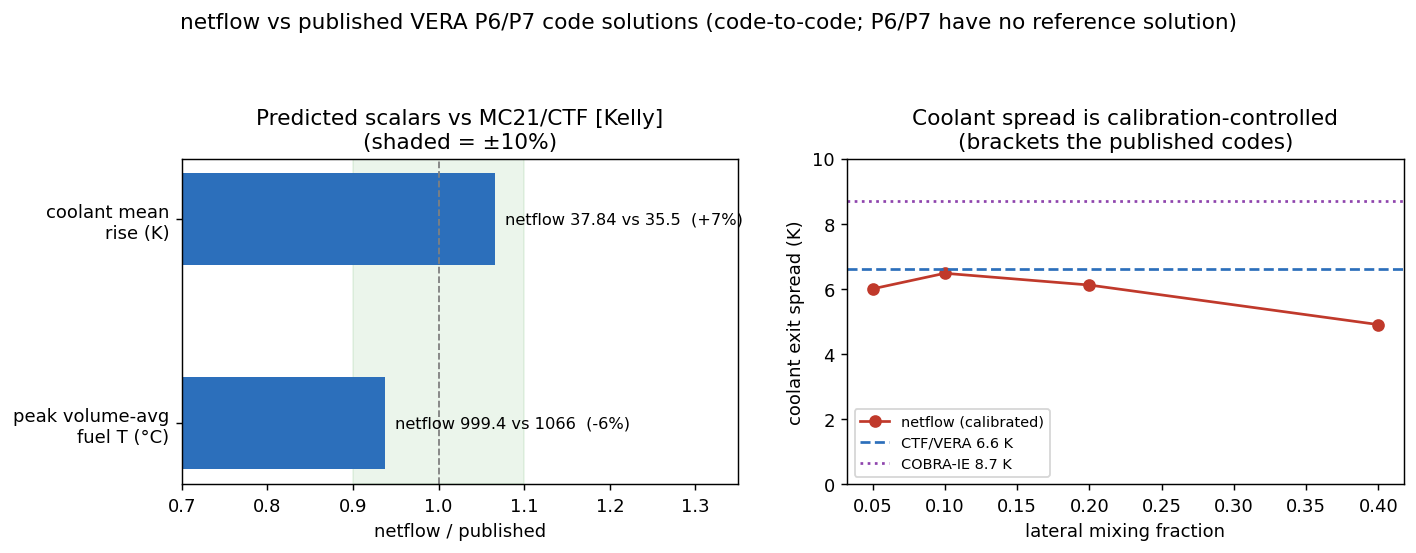
\includegraphics[width=\linewidth]{vera_comparison.png}
\caption{Code-to-code comparison, visualized. \emph{Left:} predicted scalars as
the netflow/published ratio (shaded $\pm$10\%) --- peak volume-average fuel
temperature and coolant mean rise both within ${\sim}7\%$ of the MC21/CTF
solution~\cite{kelly}. \emph{Right:} the calibrated coolant exit spread vs.\ the
lateral-mixing fraction, bracketing the published CTF/VERA (\SI{6.6}{K}) and
COBRA-IE (\SI{8.7}{K})~\cite{aviles} values --- the spread is
calibration-controlled, not predicted.}
\label{fig:compare}
\end{figure}

\paragraph{Reading the table honestly.} Fuel temperature is the strongest
comparison (Fig.~\ref{fig:compare}): netflow's peak volume-average (\SI{999}{\celsius}) lands within 6\% of
the published MC21/CTF value (\SI{1066}{\celsius}) for a single hot pin at
Problem~7's peak local peaking ($1.918$ vs.\ the published $1.92$), given the
calibrated gap conductance. The coolant mean rise matches the assembly energy
balance, $\SI{17.21}{MW}/(\dot m c_p)\approx\SI{36}{K}$. The exit spread is
\emph{not} a prediction---it is set by the cross-flow calibration---but for the
Problem~6 (single enrichment, near-flat power) assembly, sweeping the lateral
mixing fraction over $0.05$--$0.40$ gives \SIrange{4.9}{6.5}{K}, essentially
matching the MC21/CTF and VERA value (\SI{6.6}{K}) and falling under the
MC21/COBRA-IE value (\SI{8.7}{K})~\cite{aviles}. The eigenvalue row is \emph{verification}
against an analytic slab, not a P6 comparison: netflow's one-group diffusion does
not attempt the multigroup pin-resolved P6 eigenvalue ($1.16424$~\cite{kelly}),
and we do not claim it.

\paragraph{Self-consistent multiphysics (mechanism).} Coupling the neutronic and
thermal plugins through Picard with Doppler feedback ($\Sigma_a\propto\sqrt{T}$)
\emph{computes} the power distribution rather than imposing it, closing the
``power is imposed'' caveat. The coupled solve exhibits a \emph{negative}
fuel-temperature reactivity coefficient---the sign underlying inherent reactor
stability. We report this as a mechanism/sign demonstration only: it is shown on
a one-group bare slab with illustrative cross-sections, so its \emph{magnitude}
is not a physical prediction. The physical reference for fresh 3.10\,wt\%
UO\textsubscript{2}, $-2$ to $-2.5$\,pcm/K, is itself \emph{derived} by us from
the spec's reference KENO-VI eigenvalues at varied fuel temperature for
Problems~1--2~\cite{vera} (the spec reports no Doppler coefficient directly).

\section{Scope and limitations}\label{sec:scope}
\paragraph{Relationship to established acausal tools.} The abstraction here is not
new. A node carrying a \emph{potential} (across) variable and an edge carrying a
conserved \emph{flow} (through) variable, with potentials equated and flows summed
to zero at each node, is the acausal connector formalized by
Modelica~\cite{modelica} and, in Julia, ModelingToolkit~\cite{mtk} (productized as
Dyad), on the older effort/flow foundation of bond graphs~\cite{bondgraph}. Those
ecosystems are mature, symbolic, compiled, and far faster, with validated domain
libraries (e.g.\ TRANSFORM for nuclear thermal-hydraulics). \texttt{netflow} is
best understood as a \emph{minimal, transparent, pure-Python re-derivation} of
that paradigm---useful for pedagogy and dependency-light embedding, not a new
modeling capability nor a replacement for those tools.

The defining boundary: \texttt{netflow} is a scalar conservation-network solver.
Every edge flux is a function of two scalar endpoint states, and there is no
momentum equation---pressure drop is a quasi-steady loss relation, not solved
momentum. Consequences and honest growth paths:
\begin{center}
\begin{tabular}{lll}
\toprule
item & status & cost in this abstraction \\
\midrule
conductivity-integral pellet & two-node mean-$T$ now & fidelity dial (radial mesh) \\
two-phase convection / DNB & single-phase only & fidelity dial (new edge correlations) \\
transverse momentum closure & scalar pressure network & \textbf{outside} the scalar-flux abstraction \\
mechanistic gap (burnup) & fixed $h_\text{gap}$ & external correlation input \\
\bottomrule
\end{tabular}
\end{center}
The first two and the gap are fidelity dials inside the current model; transverse
momentum is the one genuine frontier. \texttt{netflow} targets fast, transparent
pre-design scoping accurate to tens of degrees, on a single core that also solves
pipe networks and criticality eigenproblems. It is not a replacement for
CTF/COBRA-TF.

\begin{thebibliography}{9}\small
\bibitem{vera} A.~T.~Godfrey, \emph{VERA Core Physics Benchmark Progression
Problem Specifications}, CASL-U-2012-0131-004, Oak Ridge National Laboratory, 2014.
\bibitem{kelly} D.~J.~Kelly III \emph{et al.}, ``MC21/CTF and VERA multiphysics
solutions to VERA core physics benchmark progression problems 6 and 7,''
\emph{Nucl.\ Eng.\ Technol.} \textbf{49} (2017) 1326--1338.
\bibitem{aviles} B.~N.~Aviles \emph{et al.}, ``MC21/COBRA-IE and VERA-CS
multiphysics solutions to VERA core physics benchmark problem \#6,''
\emph{Prog.\ Nucl.\ Energy} \textbf{101} (2017) 338--351.
\bibitem{fink} J.~K.~Fink, ``Thermophysical properties of uranium dioxide,''
\emph{J.\ Nucl.\ Mater.} \textbf{279} (2000) 1--18.
\bibitem{matpro} \emph{MATPRO / IAEA TECDOC-1496}: thermophysical properties of
materials for water-cooled reactors (Zircaloy-4 conductivity), IAEA, 2006.
\bibitem{petersen} H.~Petersen, \emph{The Properties of Helium}, Risø/DTU
Report~224, 1970.
\bibitem{dittus} F.~W.~Dittus and L.~M.~K.~Boelter, \emph{Univ.\ Calif.\ Publ.\
Eng.} \textbf{2} (1930) 443.
\bibitem{gnielinski} V.~Gnielinski, ``New equations for heat and mass transfer
in turbulent pipe and channel flow,'' \emph{Int.\ Chem.\ Eng.} \textbf{16}
(1976) 359--368.
\bibitem{todreas} N.~E.~Todreas and M.~S.~Kazimi, \emph{Nuclear Systems I:
Thermal Hydraulic Fundamentals}, 2nd ed., CRC Press, 2012.
\bibitem{scipy} P.~Virtanen \emph{et al.}, ``SciPy 1.0: fundamental algorithms
for scientific computing in Python,'' \emph{Nature Methods} \textbf{17} (2020)
261--272.
\bibitem{coolprop} I.~H.~Bell \emph{et al.}, ``Pure and pseudo-pure fluid
thermophysical property evaluation and the open-source thermophysical property
library CoolProp,'' \emph{Ind.\ Eng.\ Chem.\ Res.} \textbf{53} (2014)
2498--2508.
\bibitem{modelica} Modelica Association, \emph{Modelica Language Specification},
v3.x; see also P.~Fritzson, \emph{Principles of Object-Oriented Modeling and
Simulation with Modelica}, 2nd ed., Wiley, 2014.
\bibitem{mtk} Y.~Ma \emph{et al.}, ``ModelingToolkit: A Composable Graph
Transformation System for Equation-Based Modeling,'' arXiv:2103.05244 (2021).
\bibitem{bondgraph} D.~C.~Karnopp, D.~L.~Margolis, R.~C.~Rosenberg, \emph{System
Dynamics: Modeling, Simulation, and Control of Mechatronic Systems}, 5th ed.,
Wiley, 2012 (effort/flow bond graphs, after H.~M.~Paynter, 1961).
\end{thebibliography}

\end{document}
